\documentclass[11pt]{article}


\usepackage[utf8]{inputenc}
\usepackage[english]{babel} % language
\usepackage{graphicx} % images
\usepackage{float} % images
\graphicspath{ {./img/} } % images default path
% setting document style
\usepackage[a4paper,
            bindingoffset=0.2in,
            left=1in,
            right=1in,
            top=1in,
            bottom=1in,
            footskip=.25in]{geometry}
\usepackage{listings}





\begin{document}
\begin{titlepage}
    \thispagestyle{empty}
    \newcommand{\HRule}{\rule{\linewidth}{0.5mm}}
    \hspace{1cm}
    \center
    
    \textsc{\huge University of Milano-Bicocca}\\[0.5cm]
    
    \begin{center}
		\includegraphics[scale = 0.25]{logoUnimib.png}\\[2cm]
	\end{center}
    
    \textsc{\LARGE Text Mining and Search\\
    \Large Final project}\\
    
    \HRule\\[0.5cm]
    { \huge \bfseries Classification and clustering techniques on amazon fine food reviews} 
    \HRule \\[2cm]
    
    \begin{center}
    	\textbf{Authors:}\\
    	Confalonieri Riccardo, 830404, r.confalonieri5@campus.unimib.it\\
    	Ranieri Silvia, 878067, s.ranieri7@campus.unimib.it
    \end{center}
    
    \vspace{7cm}
    
    \begin{center}
    	A.Y.: 2021/2022
    \end{center}
\end{titlepage}

\thispagestyle{empty}
\pagenumbering{gobble} 
  \tableofcontents


\clearpage
\setcounter{page}{0}
\pagenumbering{arabic}
\setcounter{page}{1}

\begin{abstract}
Amazon is the most popular e-commerce site in the world, as well as the largest internet company with a market cap of 1,668 billion dollars in 2020. One of its greatest strengths is the review system that allows each customer to express positive opinions or complaints about purchased products. \\
This project, starting from fine food reviews, focused on two different tasks: in the first has been implemented classification models to determine the opinion of users, both in binary and multi-class format, the second task instead is focused on unsupervised clustering model. All these tasks were preceded by a phase of pre-processing and representation of the text. Finally, as an additional task, an unsupervised approach to extract the most relevant topics present in the reviews has been considered.\\
The results obtained in the first task were found to be quite satisfactory in the binary case, unlike the more complex case of the multiclass classification. Similarly, in clustering, ideal results were not obtained even if from a semantic point of view the results are slightly better. The attempt at topic modeling, on the other hand, gave good results even with a very basic approach. 
\end{abstract}


\section{Introduction}
Amazon reviews are known all over the world and are a key element to improve the visibility of their products on the platform.
Over the years this review system has become more and more organized and is a strong influencer during purchases, in fact customers find in these reviews genuine opinions given by other users similar to them. Half of all online consumers seems to rely mainly on product reviews before buying them. On the other hand also sellers has some advantages because if products receive positive reviews will appear higher on the page and therefore is more likely to be sold. In this scenario, it is clear the importance of an automated system that checks if the assigned score corresponds to the reivew's written text, in order to prevent the use by vendors of automatic bots or other techniques to obtain positive reviews for their products. In this sense, amazon's decision to eliminate famous sellers for false positive reviews has made news in the last period.
For this reason, as main tasks, it was decided to implement a classification model and a clustering model. 
The goal is to look for models that can actually be valid and that, given a new review, can verify if the score assigned by the user is consistent. Ideally, with efficient models, the process of assigning the score could be automated, leaving the user only the possibility to write the review, in doing so you would have reviews and evaluations that are as consistent and valid as possible for everyone.

\section{Dataset}
The data used for the project are strongly based on the text and numerical evaluation (score) of the reviews. Specifically the data used was downloaded from kaggle \cite{kaggleDataset} and consists of reviews of fine foods from amazon. The features present in our dataset are:
\begin{itemize}
    \item ProductId. Unique identifier for the product.
    \item UserId. Unique identifier for the user.
    \item ProfileName. Profile name of the user.
    \item HelpfulnessNumerator. Number of users who found the review helpful.
    \item HelpfulnessDenumerator. Number of users who indicated whether they found the review helpful or not.
    \item Score. Rating assigned to the review between $1$ and $5$.
    \item Time. Review date in UNIX format.
    \item Summary. Brief summary of the review.
    \item Text. Text of the review.
\end{itemize}
From the statistical analysis it emerged that our dataset contains $568454$ reviews made by over $200$k users about $74258$ products. All of these reviews were collected between August 1999 and October 2012.\\
The first analyzes on the dataset highlighted some problems on the raw data downloaded that required some manipulation and cleaning phases before actually starting with the NLP tasks. First of all there are \textit{duplicated reviews} in the dataframe, duplicated reviews are those made by the same user id with the same rating, time and text but different product code. This can be due to many factors such as different sellers or amazon policies, however since the text and rating are the same it was decided to delete them anyway because they would not add useful data for the classification (same characteristics). This because it is difficult that a consumer purchase multiple identical products at the same time from different sellers, so it is reasonable to assume that it is precisely the same review that is automatically duplicated. Moreover has been noticed that some reviews have only the same user id and the same product id. Those reviews could be motivated by multiple purchase in different time or by an update of the first reviews maybe after the seller has answer to some faced problems. The first case could be usefull for NLP task because contains different features but sometimes those rows contains even the same text and only a different score, probably it is the update cases and this can be a problem for next tasks. For these reasons, and for not selecting by hand each reviews, all this rows has been deleted and only the most recent ones has been keeped. After those removals the dataset contains $392969$ reviews. Then has been noticed that some summaries contain \textit{null values}, as this column will not be considered further a simple fill replace has been applied. \\
After has been observed that there was a \textit{strong imbalance in the ratings score} as you can see in Figure \ref{scoreImb} below. This imbalance can cause errors in the fitting of the models and therefore it will be necessary to manage it correctly for the portion of the dataset that will be used as training. Instead it is good to keep this unbalanced distribution in the test portion that will be used to evaluate the different models as it reports a real situation supposed to be real. 
\begin{figure}[H]
\begin{center}
  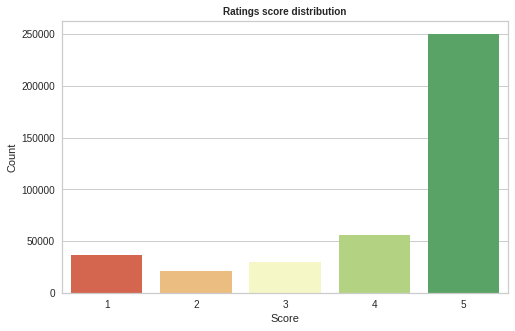
\includegraphics[scale = 0.55]{imbalance.png}
  \caption{Reviews per score}
  \label{scoreImb}
\end{center}
\end{figure}
\noindent Finally the \textit{temporal shifting} has been studied and no evidence of different text styles has been found so all rows has been keeped. During this analysis has emerged that reviews with \textit{score equal to 5 shows the greatest growth among all scores}, this seems unusual and one might wonder that people are generally optimistic or most likely there are unverified accounts that are increasing the seller inappropriately with fake reviews as happened in recent years. Again all rows has been keeped due to the fact that in the dataset is not reported any form of authenticity for each reviews. At this point the dataset is ready to be preprocessed and used for the NLP tasks.

\section{Preprocessing}
To proceed with the analysis, the preprocessing part was necessary for uniform all texts. Never the less it's correct implementation is not easy and can be different for each dataset. Each preprocessing phases made in this project will be explained in details in the next subsections.

\subsection{Normalization and special characters}
It is an operation of pre-treatment of the text that allows to eliminate the ambiguities present in the fragments of the corpus. It is the first applied phase because usually packages for stopwords removal and stemming are based on a pre-defined set of words. Never the less this set of words is usually in lowercase fold and also does not consider strange accents that maybe some user can add in his reviews. 
So starting from this consideration the considered steps are:
\begin{enumerate}
    \item Lowercase conversion of all texts.
    \item Abbreviation replacement.
    \item Accents replacement.
\end{enumerate}
Abbreviation replacements has been applied to preserve the word `not' because it could be very important for qualifying correctly binary reviews. Since there is not a predefined dictionary to expand common abbreviations the focus has been only to the most common forms of abbreviating `not' that has been expanded by using regex's (e.g `don't' will be expanded to `do not'). The accent replacements treatment do more or less the same with accent syllables by replace them with the standard syllable (e.g. `ò' will be `o').

\subsection{Specific preprocessing for this dataset}
By inspecting the results after the normalization step can be notice that the dataset contains some specific issues:
\begin{itemize}
    \item presence of URLs and/or HTML tags.
    \item presence of URLs written in text format such as: www(dot)francescorinaldi(dot)com
    \item presence of textual emojis (e.g. :) ).
    \item presence of multi spaces.
    \item presence of numbers and puntuactions.
\end{itemize}
All this problems has been solved by defining custom regex for cleaning each text. 

\subsection{Stopwords}
Stopwords are common words of a text, those that have nothing to do with a specific topic. Since these words can be used in any context they are not significant and therefore their removal allows to obtain more accurate models. However there is no single list of stopwords, in this project it was decided to use the default one provided by the nltk package. As said before the word `not' as been removed from this common list while specific context words like `product' and `Amazon' has been added to the list.

\subsection{Tokenization and Stemminig}
Tokenization's goal is to divide a text flow into meaningful units called tokens. This is very important either for applying stemming techniques either for text representation.
The choice of applying stemming instead of lemming was taken considering that stemming technique is effective in our case because the reduction process did not lose information and the root of the word has kept the same thematic meaning of the complete form. Furthermore the dataset contains a huge words and so the lemmatization technique requires very long computational time and great hardware resources.

\section{Handling score imbalance}
After the preprocessing phase all the dataset has the same text characteristics but the score columns is still highly imbalanced. Again, this is a problem only for training data due to the fact that the test set should preserve the unbalance because in this way it can simulate what it will happens in a real situation and so get a real score of the model. \\
Before splitting the dataset, as has been decided to apply a binary classification, it is necessary to apply some further transformations to the dataset:
\begin{itemize}
    \item Delete all columns with a neutral score (i.e. Reviews with score equal to $3$).
    \item Convert the remaining scores into two different class \textit{positive}, that represent reviews with score equal to $4$ or $5$, and \textit{negative} with score equal to $1$ or $2$. For simplicity, these two classes will be represented in a binary way so the positive class will be indicated as  $1$ and the negative class with $0$.
\end{itemize}
Of course this score conversion could not be the optimal one but is an approximate and proxy way of determining the polarity (positivity/negativity) of a review. After this steps the data was divided into two subset: training and test, in particular $20\%$ of rows were kept as test set to evaluate the models. To deal with the initial problem of score unbalancing, once the sets were divided, the downsampling technique was applied for the majority class of the training set to have an equal number of instances for both negative and positive reviews. Specifically the training is made by $45633$ examples for each binary score. \\
It is important to remember that all preprocessing steps has been already applied on both training and test set, otherwise before using the test set it would be necessary to apply the same steps for getting comparable texts!

\newpage
\section{Text Representation}
Before applying the text representation the length of each reviews has been analyzed, it emerged that the most reviews has more or less the same number of words so even a simple representation could be valid. For this reasons, at the beginning, has been decided to apply this two techniques:
\begin{itemize}
    \item Bag of words (BOW). Specifically it counts the number of occurrences of each words and not only their presence or absence.
    \item TF-IDF. 
\end{itemize}
Both this extracted representations contains a very large number of features ($12135$), this requires high resources and computational time to be able to classify and group the data. For this reason the Truncated SVD techniques as been applyied to reduce the number of features, the choosen of this technique instead of the standard SVD is driven by the fact that is most suitable for working with sparse matrix as the ones obtained from BOW and TF-IDF. In particular the Truncated SVD has been setted to try to minimize the number of features while maintaining more or less 75\% of the explained variance.
The explained variance values and the number of features extracted for each representation are shown in the table below:
\begin{table}[H]
    \begin{center}
        \begin{tabular}{||l||c|c||}
            \hline
            Techniques & Explained var. & \#Features\\
            \hline
            \hline
            BOW & $0.756$ & $600$\\
            \hline
            TF-IDF & $0.737$ & $1500$\\
            \hline
        \end{tabular}
    \caption{Explained variance per representation techniques}
    \end{center}
\end{table}


\section{Classification task}
The first NLP task considered, after the text representation phase, is the classification task that is a supervised machine learning task. Specifically, this task was approached with two different purposes: 
\begin{itemize}
    \item Binary classification. The first task try to classify reviews into two macro categories: positive (label $1$) and negative (label $0$).
    \item Multiclass Classification. This second task try to predict the real score in the range $[1,5]$ by using a modern approach with recurrent neural networks and word embeddings.
\end{itemize}


\subsection{Binary classification}
As mentioned previously, the goal is to classify reviews into two macro categories: positive or negative. To solve this task different types of classification models has been developed, each one has been fitted with both the the two text representations described above to understand if there are some differences. First models that has been considered are:
\begin{itemize}
    \item Logistic regression.
    \item Support vector machine (SVM).
    \item Light LGBM classifier.
\end{itemize}
Each of this classifier has been evaluated on the same test set in order to be comparable, for choosing the best model the macro-average F1-score is calculated and compared. This metric was used as it also considers the recall of the two classes in addition to the precision. Furthermore, the macro-average version is used as the test set has been kept unbalanced and therefore this metric reports more information in a single number than the simple accuracy. Now each classifier will be analyzed more in details.

\subsubsection{Logistic regression}
Logistic regression basically it is a linear classifiers that assign a probability between $0$ and $1$ for each class, with a sum of one. To predict which class a data belongs, a threshold can be set. Based upon this threshold, the obtained estimated probability is classified into classes. The default threshold value, that has also been used in this project, is $\geq 0.5$ so if the predicted value if greater than this threshold the data belongs to the positive reviews class.\\
With this classifier the TF-IDF representation achieve best results, as you can see from the comparison report on test set reported in Figure \ref{logreg_fig} below. By focusing only on the macro avg metrics you can see that this model is quite good but if you look more closely at the confusion matrix you can see that several positive reviews are misclassified as negative. Furthermore, comparing the training and test results, the model seems to overfill during the training phase precisely on the `negative' class. Furthermore, despite the fact that the classification is quite good, analyzing the top-$10$ most informative features used by the model, reported in Table \ref{logreg_t1} and \ref{logreg_t2},  you can notice how the words do not seem to be very informative.
\vspace{1cm}

\begin{figure}[H]
	\begin{minipage}[b]{0.48\textwidth}
		\centering
		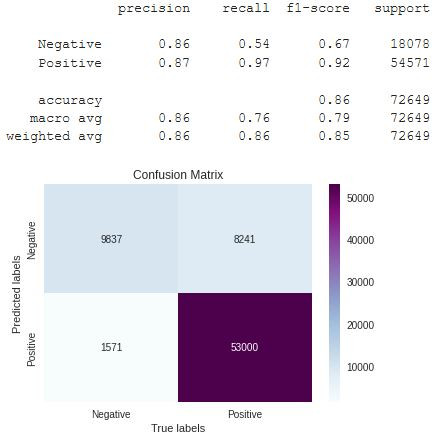
\includegraphics[width=\textwidth]{logreg_bow.JPG}
		{Results of logistic regression on BOWs}
	\end{minipage}
	\hfill
	\begin{minipage}[b]{0.48\textwidth}
		\centering
		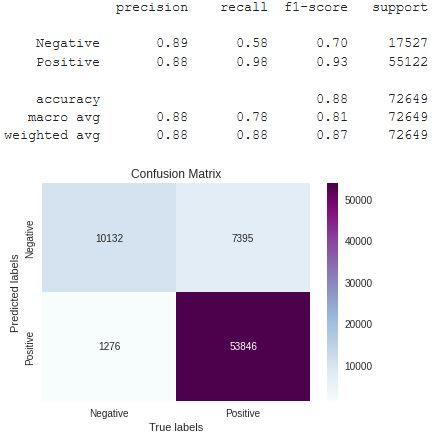
\includegraphics[width=\textwidth]{logreg_tfidf.JPG}
		{Results of logistic regression on TF-IDF}
	\end{minipage}
	\caption{Logistic regression comparison on same test set}
	\label{logreg_fig}
\end{figure}
\vspace{0.5cm}
\hspace{-2cm}
\begin{minipage}[b]{0.48\textwidth}
        \begin{table}[H]
            \begin{center}
                \begin{tabular}{||c||c|c|c||}
                    \hline
                    Score & Neg. Words & Score & Pos. Words\\
                    \hline
                    \hline
                    $-1.86$ & abl & $1.27$ & antisept \\      \hline
                	$-1.59$ & advertis & $1.24$ &	acut\\          \hline 
                	$-1.43$ & abhor & $1.12$ & aesthet\\        \hline
                	$-1.22$ & abund & $1.12$ & achiev\\         \hline
                	$-1.04$ & apiec & $1.07$ & aafco\\          \hline
                	$-0.99$ & apex & $1.04$ & aggrav\\         \hline
                	$-0.97$ & arginin & $1.03$ & abid\\           \hline
                	$-0.96$ & acidophilu & $1.01$ & adventuresom\\   \hline
                	$-0.96$ & accessori & $1.00$ & anti  \\         \hline
                	$-0.94$ & apart & $0.99$ & alik\\        \hline
                    \hline
                    \hline
                \end{tabular}
            \caption{Top-10 most informative features logistic regression on BOWs}
            \label{logreg_t1}
            \end{center}
        \end{table}
\end{minipage}
\hspace{2cm}
\vspace{25pt}
\begin{minipage}[b]{0.48\textwidth}
    \begin{table}[H]
        \begin{center}
            \begin{tabular}{||c||c|c|c||}
                \hline
                Score & Neg. Words & Score & Pos. Words\\
                \hline
                \hline
                $-9.50$ & abysm & $37.23$ & aback  \\   \hline     
            	$-7.03$ & act & $9.95$ & abl    \\         \hline
            	$-6.05$ & abroad & $8.86$ & acai     \\       \hline
            	$-5.69$ & accomod & $7.81$ & absorpt  \\       \hline
            	$-5.45$ & address & $7.73$ & acquir   \\       \hline
            	$-5.25$ & ace & $6.81$ & advis    \\       \hline
            	$-4.62$ & aberr & $6.56$ & advantag \\       \hline
            	$-4.51$ & anim & $6.26$ & acv   \\          \hline
            	$-4.38$ & acclim & $6.16$ & anoth \\          \hline
            	$-4.25$ & appli & $6.13$ & across\\ \hline
                \hline
                \hline
            \end{tabular}
        \caption{Top-10 most informative features logistic regression on TF-IDF}
        \label{logreg_t2}
        \end{center}
    \end{table}
\end{minipage}

\subsubsection{Support vector machine (SVM)}
The second types of classifier that has been deviloped is an SVM. The classic SVM classifier cannot be applied due to the complexity of the data, so an approximate version that allows very fast execution times has been used. However, as you can see from figure \ref{svm_fig} the results are much worse than before, and moreover it maintains the same problems of the previous classifier, that is a strong overfitting in the `negative' class as well the top-10 most informative features are again not so good. 
\begin{figure}[H]
	\begin{minipage}[b]{0.48\textwidth}
		\centering
		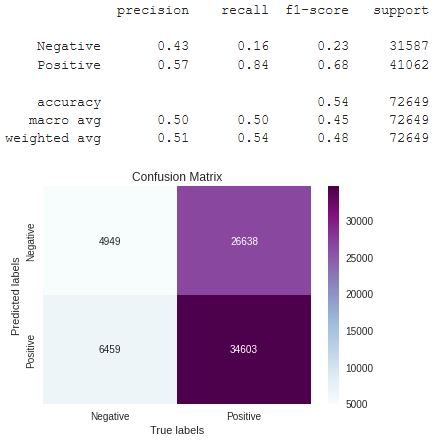
\includegraphics[width=\textwidth, height = 6.5cm]{svm_bow.JPG}
		{Results of approximate SVM on BOWs}
	\end{minipage}
	\hfill
	\begin{minipage}[b]{0.48\textwidth}
		\centering
		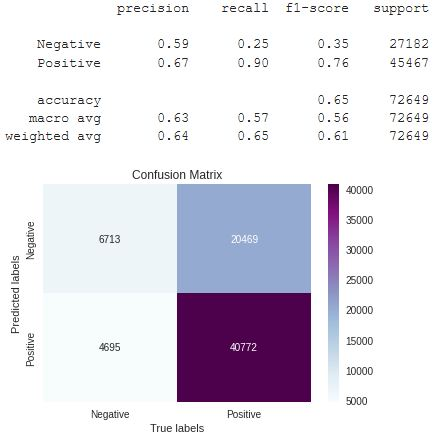
\includegraphics[width=\textwidth, height = 6.5cm]{svm_tfidf.JPG}
		{Results of approximate SVM on TF-IDF}
	\end{minipage}
	\caption{Approximate SVM comparison on same test set}
	\label{svm_fig}
\end{figure}

\subsubsection{Light LGBM}
The last classifier that has been tried is a different one. This is a very fast, distributed, high performance gradient boosting framework based on decision tree algorithms. So it works in slight different ways with respect to the previous classifiers. Unfortunately this classifier did not give the desired results, it turned out to be better than the approximate SVM but still slightly worse than the logistic regression. And as in the previous cases it is subject to overfitting with respect to the `negative' class.
\begin{figure}[H]
	\begin{minipage}[b]{0.48\textwidth}
		\centering
		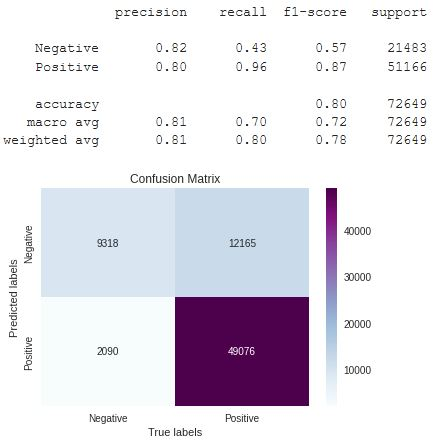
\includegraphics[width=\textwidth]{light_bow.JPG}
		{Results of light LGBM on BOWs}
	\end{minipage}
	\hfill
	\begin{minipage}[b]{0.48\textwidth}
		\centering
		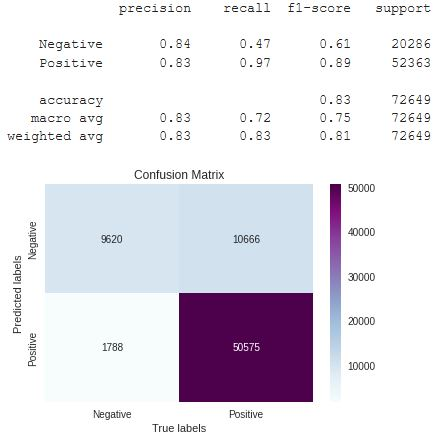
\includegraphics[width=\textwidth]{light_tfidf.JPG}
		{Results of light LGBM on TF-IDF}
	\end{minipage}
	\caption{Light LGBM comparison on same test set}
	\label{light_fig}
\end{figure}

\subsubsection{N-grams TF-IDF}
The TF-IDF representation is the one that has given the best results so far, however the most representative words do not seem to be the best possible. Analyzing the poorly classified sentences it emerged that many contained the word `not', for this reason has been tried to represent the texts using n-grams TF-IDF with $n = 2$. The classifier used in this case is logistic regression which resulted be the best. With this new configuration it was possible to slightly improve the results, as you can see in the Figure \ref{ngrams_fig}, and even the most significant words turn out to be much better, even if not perfect (e.g. `not' as single words is the second most discriminant negative word.) as you can see in the table \ref{ngrams_t}.

\hspace{-2cm}
\begin{minipage}[b]{0.48\textwidth}
\centering
\begin{figure}[H]
\begin{center}
  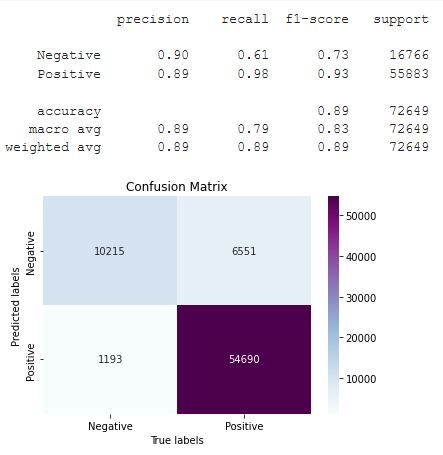
\includegraphics[scale = 0.55]{img/logreg_ngrams.JPG}\\
  \caption{Results of logistic regression on bi-grams TF-IDF}
  \label{ngrams_fig}
\end{center}
\end{figure}
\end{minipage}
\hspace{1cm}
\begin{minipage}[b]{0.48\textwidth}
    \begin{table}[H]
        \begin{center}
            \begin{tabular}{||c||c|c|c||}
                \hline
                Score & Neg. Words & Score & Pos. Words\\
                \hline
                \hline
                $-13.87$ & disappoint & $13.58$ & great   \\ \hline       
            	$-10.37$ & not & $11.42$ & delici     \\ \hline    
            	$-9.77$ & not recommend & $11.30$ & best        \\ \hline   
            	$-8.89$ & worst & $10.65$ & love        \\ \hline   
            	$-8.64$ & not good & $9.84$ & perfect     \\ \hline   
            	$-8.51$ & not buy & $9.20$ & good         \\ \hline  
            	$-8.02$ & not worth & $8.85$ & not disappoint \\ \hline
            	$-7.63$ & terribl & $8.11$ & excel      \\ \hline    
            	$-7.43$ & unfortun & $7.27$ & favorit   \\ \hline     
            	$-7.35$ & aw & $7.10$ & nice \\ \hline
                \hline
                \hline
            \end{tabular}
        \caption{Top-10 most informative features logistic regression on TF-IDF}
        \label{ngrams_t}
        \end{center}
    \end{table}
\end{minipage}

\subsection{Multiclass Classification}
The previous task considers only positive and negative reviews. This second classification task try to carry out a multi class classification by predicting the real score in the [1,5] range.
In this case a modern approach has been tried by using a recurrent neural network, specifically the long short term memory network (LSTM) with an embedding layer. Before training this network, since this task is little difference then before, it is necessary to split again the dataset without converting the score column and applying the same techniques for balancing the training set class. After this steps the training set contains  more than $16000$ examples per class, from this set has been extracted a random $10\%$ of samples as validation set during the training phase.\\
However, this model did not give the desired results and is subject to an accentuated overfitting between training and validation set. As can be seen from the figure \ref{lstm}, which reports the evaluation of the model on the test set, the classification of the $4$ and $5$ scores is often confused. While for the neutral class ($3$) the greatest number of instances are correctly classified but here too there are errors and very often it is classified with a score equal to $4$. Finally, you can note that the class $1$ is the one with the most errors, and above all the score is often confused with diametrically opposite values equal to $4$ or $5$, thus classifying the review as positive rather than negative. The classification of the score in the range $[1,5]$ starting from the text was therefore not a simple task even using a modern approach. A possible improvement could be to consider a pretrained model like Word2Vec or Glove to embed the texts, in this way the context of the words would be taken into account as well. 
\begin{figure}[H]
\begin{center}
  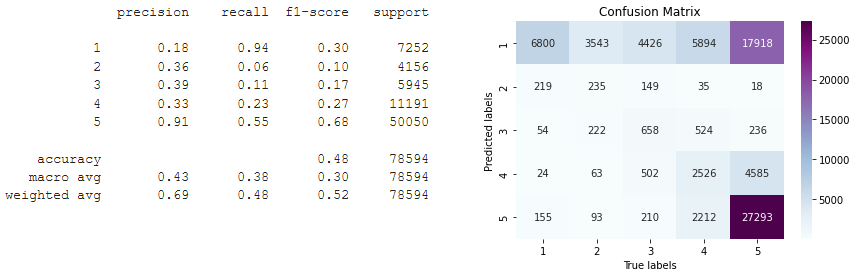
\includegraphics[scale = 0.6]{img/LSTM.png}\\
  \caption{Results of LSTM with word embeddings}
  \label{lstm}
\end{center}
\end{figure}


\section{Clustering}
The second application of NLP activity is clustering. Even for this task two different approach has been investigated:
\begin{enumerate}
    \item partition the texts into $5$ groups to check if cluster membership could correspond to the review score.
    \item partition texts by selecting the number of groups to maximize a clustering metric.
\end{enumerate}
Both this approaches has been represented with TF-IDF, but as the values distribution could negatively affect clustering identification a standardization technique was applied. This is not strictly required by models but can be very useful especially with classical distances such as the Euclidean one, this because if one of the our feature has a much wider range of values than the others, clustering will be completely dominated by that feature.\\
Subsequently, keeping the score as target variable, using T-SNE the number of features considered was reduced to two, in this way it was possible to view the features in 2D space.
For computational problems, the reduction was carried out only on a sub-portion of $500$ reviews, this highlighted how the reviews do not seem to assume a specific position and therefore it is difficult to obtain clusters with valid scores if the classic evaluation measures are used. 

\subsection{Clustering in $5$ groups}
As mentioned before this approach try to clustering the data into $5$ different groups. The goal is to to find clusters that contain a specific score. For carrying out this task two different models has been tried: \textit{k-means} and \textit{hierarchical clustering}. Both of these approaches were evaluated with the adjusted mutual information score which also takes into account the number of clusters. This metric is also independent of the absolute values of the labels: a permutation of the class or cluster label values won’t change the score value in any way. By comparing the clustering label with the score label (ground truth) the results was not satisfactory, k-means reach $0.0080$ and hierarchical $0.00112$. In addition to giving worse results, the hierarchical method requires particular memory management and therefore it was not possible to use all the data available but only a subset of them.\\
The results of this approach were also evaluated by a semantic point of view through wordclouds, so as to verify if the data had been grouped with respect to their textual content. Even in this case the result seems to be not so good. In particular, with the exception of cluster $1$ which seems to talk about food, the different clusters contain repeated terms such as `flavor' and `taste', so that even in this respect the grouping does not seem to obtain the desired results. Figure \ref{cluster_5_fig} shows the wordclouds extracted from k-means clustering, in the hierarchical case the result is slightly worse but the same considerations apply. 
\begin{figure}[H]
\begin{center}
  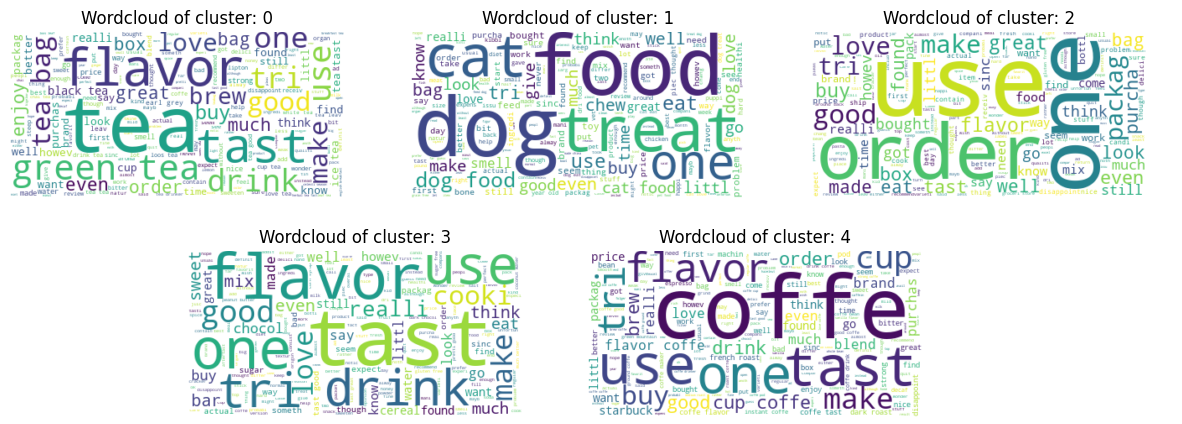
\includegraphics[scale = 0.5]{img/cluster_5.png}\\
  \caption{Wordclouds extracted from k-means with k = 5}
  \label{cluster_5_fig}
\end{center}
\end{figure}


\subsection{K-means on optimal number of cluster}
Finally, the k means method was applied by maximizing the silhouette metric to find the optimal number of clusters which turned out to be $10$. The goal is to form clusters that divides the content of the reviews.
Of course in this case is not possible to evaluate groups with some ground truth label so semantic evaluation with wordclouds has been carried out. 
The result is this case is quite satisfying. By analyzing figure \ref{cluster_10_fig} you can see that some rough division exists in clusters. For example, cluster $8$ appears to be talking about chocolate/snacks/sugar, cluster $6$ is clearly about tea, etc. However, some clusters seem to report the same themes as cluster $3$ and $7$. This was expected because even if the the silhouette index was maximized it remains close to zero.

\begin{figure}[H]
    \hspace{-29.5pt}
    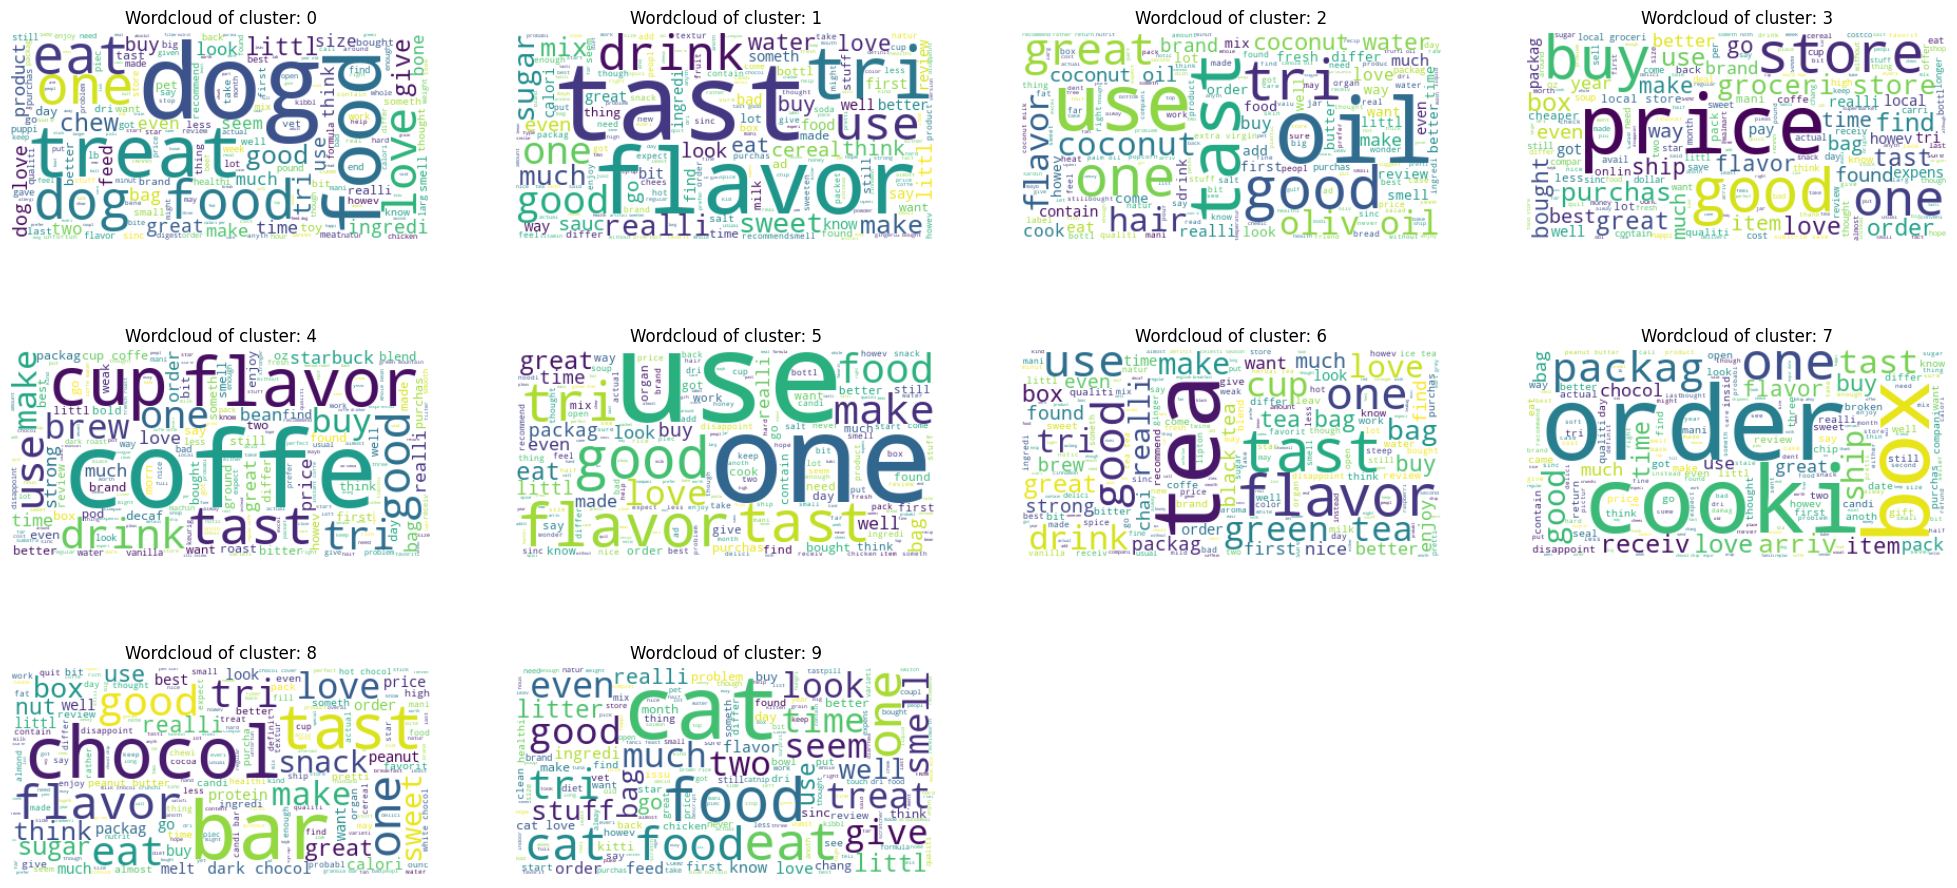
\includegraphics[scale = 0.35]{img/cluster_10.png}\\
    \caption{Wordclouds extracted from k-means with k = 10}
    \label{cluster_10_fig}
\end{figure}

\section{Topic Modeling}
As an additional task the LDA (Latent Dirichlet Allocation) topic modeling has been tried to carry out. This is unsupervised learning, because it automatically groups words without a predefined list of labels.
The presence of at least $5$ topics had already emerged from the previous clustering: animals, coffee, tea, orders, chocolate/snacks. Therefore a number of topics  $\geq 5$ that would minimize the perplexity metric has been searched, this minimization confirmed that the optimal choice for the extraction of topics is to keep $5$ different components. The results in this case are much better, by using the pyLDAvis library that allows to graphically view the topics you can see that the $5$ topics are far from each other as you can see in figure \ref{top_mod_pyLDAvis}.
\begin{figure}[H]
\begin{center}
  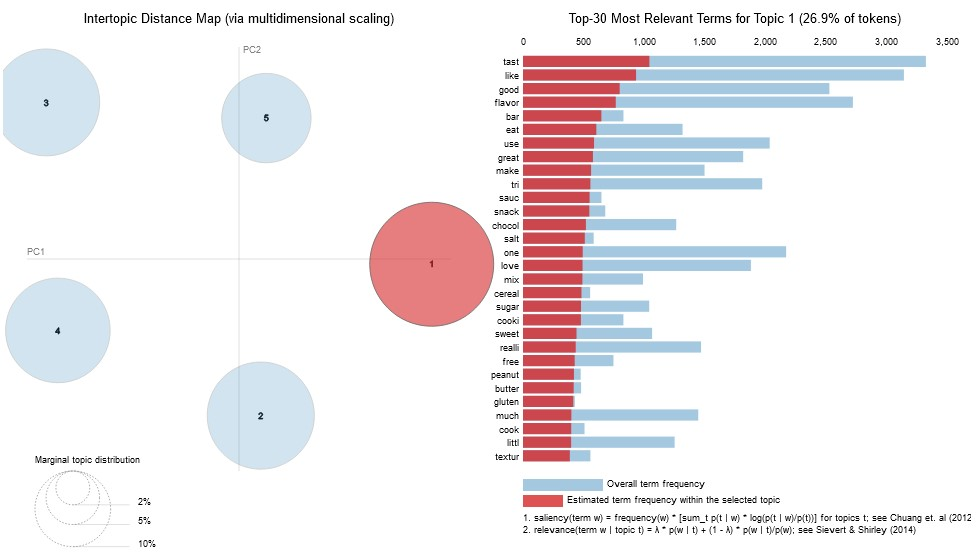
\includegraphics[scale = 0.5]{img/LDA.jpg}\\
  \caption{Visualization of topic with pyLDAvis}
  \label{top_mod_pyLDAvis}
\end{center}
\end{figure}
\noindent By default topics are marked with a number and not with the argument, so it is necessary to inspect the words contained in each one to manually assign the reference argument. By looking for each topic in the visualization proposed above with $\lambda = 1$ you can see that all topics are interpretable and even if there are words repeated or slightly out of context, it is possible to understand well the probable argument covered by each topic. About this, topic $1$ talks about general flavor and sweets, topic $2$ is about the order and shipping process, topic $3$ is for animals, topic $4$ for tea and topic $5$ talks about coffee. This interpretation remains valid even if you decrease the $\lambda$ to include also more rare words. As said before this is not perfect but seems to be quite reasonable as results.

\section{Conclusion}
By a general point of view all those tasks highlighted that the TF-IDF representation works better than a simple BOW, moreover for some task, such as the multiclass classification, n-grams representation achieve better results.
More in details, regarding the classification task the results in the binary prediction were found to be quite satisfactory, however it is possible consider more complex models or by increasing the number of neighboring words considered for n-grams for trying to improve the performance. The multiclass classification, on the other hand, highlighted various limits due to the fact that evidently there is no clear relationship between the text and the score assigned to it. However, you could try to optimize the network hyperparameters or, as already mentioned, consider pretrained models for word embeddings.
Concerning the clustering task turned out to be more complex, also due to the complexity on evaluating it. Reviews seems hardly belonging to a specific group both from the point of view of the score and from the semantic point of view, even if this second aspect gave slightly better results. Finally, the quick test done with topic modeling have shown how the topics are linked to the different categories of fine food, giving satisfactory results. 
In general is it possible to say that starting from the text models are able to predict if it is a positive or negative reviews and it's topic with good performance, but is difficult to have a completed automated model for checking a given score (or predict it). \\
For the future would be interesting to have more information about the dataset, for example to know if a reviews is verified or not since as highlighted in the initial analysis on the dataset there is a suspicious increase in positive reviews that could influence the analyzes.



\newpage
%\section*{References}
\bibliographystyle{IEEEtran}
\nocite{*}
\bibliography{references.bib}

\end{document}
